\section{Orchestration Goals and Problem Statement}

\mnote{Application function results}
To recapitulate, an application function $\appfunction{\orcfunction{\transformationset{T}}}$ for transformation networks, as defined in \autoref{def:applicationfunction}, accepts models and changes to them and yields either a tuple of models or $\bot$.
Whenever it returns a tuple of models, they must be the result of applying the transformations in $\transformationset{T}$ of the network in an order determined by the orchestration function $\orcfunction{\transformationset{T}}$.
We then say that this execution order is an \emph{orchestration} of the transformations and that the execution of transformations in that order \emph{yields} those models.
The notion of correctness for the application function given in \autoref{def:applicationfunctioncorrectness} additionally requires the returned models to be consistent.
We did, however, not yet define when we expect the function to return consistent models and when we allow it to return $\bot$, as this requires a further discussion of the alternatives, which we provide in the following.

\mnote{Dependence on orchestration function}
The application function highly depends on the results of the orchestration function.
If that function does not deliver an orchestration that yields consistent models, a correct application function may only return $\bot$.
Thus, we are particularly concerned with ensuring that the orchestration function finds an orchestration that yields consistent models as often as possible.
We call an orchestration that yields consistent models a \emph{consistent orchestration}.
Precisely, we define an orchestration and a consistent orchestration as follows.
\begin{definition}[Orchestration]
    Let $\transformationset{T}$ be a transformation set.
    We call a sequence $\sequenced{\transformation{t}_{1}, \transformation{t}_{2}, \dots} \in \transformationset{T}^{< \mathbb{N}} \equalsperdefinition \bigcup_{i=0}^{\infty} \transformationset{t}^i$ of these transformations an \emph{orchestration} of them.

    For models $\modeltuple{m} \in \metamodeltuple{M}$ and changes $\changetuple{\metamodeltuple{M}} \in \changeuniverse{\metamodeltuple{M}}$, we say that an orchestration $\sequenced{\transformation{t}_{1}, \dots, \transformation{t}_{n}}$ is \emph{consistent} if, and only if, the subsequent application of the transformations to $\modeltuple{m}$ and $\changetuple{\metamodeltuple{M}}$ is consistent, i.e.:
    \begin{align*}
        &
        \exists \changetuple{\metamodeltuple{M}}' \in \changeuniverse{\metamodeltuple{M}} : 
        \big(
            \generalizationfunction{\metamodeltuple{M},\transformation{t}_{n}} \concatfunction \dots \concatfunction \generalizationfunction{\metamodeltuple{M},\transformation{t}_{1}}(\modeltuple{m}, \changetuple{\metamodeltuple{M}}) = (\modeltuple{m}, \changetuple{\metamodeltuple{M}}') \\
            & \formulaskip
            \land \changetuple{\metamodeltuple{M}}'(\modeltuple{m}) \consistenttomath \transformationset{T}
        \big)
    \end{align*}
\end{definition}

\mnote{Length of orchestrations}
The definition of an orchestration function allows it to determine an arbitrarily long sequence of transformations, also including each transformation multiple times.
We have introduced this general notion to avoid unnecessary restrictions.
In the following, we show the necessity of having this unrestricted notion rather than allowing each transformation to be executed only once, as proposed in existing work~\cite{stevens2020BidirectionalTransformationLarge-SoSym}.
From the insight that we need to allow transformations to be executed multiple times, we derive and discuss when we expect the application function to return consistent models to finally come up with a notion of \emph{optimality} for the orchestration function determining the execution order.
This leads to the definition of the central \emph{orchestration problem} that we want a transformation network to solve.


\subsection{Single Transformation Execution}

\mnote{Ranges for executions times}
The possible numbers of executions for transformations of a network range from a selected execution of a subset, e.g., in terms of an induced spanning tree, over the execution of each transformation for one or a fixed number of times, to an arbitrary number of executions per transformation.
In the following, we demonstrate why a single execution of each transformation is not sufficient in practice and prove that it is not sufficient in general.

\mnote{Spanning trees insufficient}
The even stronger restriction to spanning trees is obviously insufficient.
Consider the following consistency relations. For simplicity reasons, we use model-level relations (\autoref{def:modellevelconsistencyrelation}) instead of fine-grained ones:
\begin{align*}
    & 
    \consistencyrelation{CR}{12} = \setted{\tupled{\model{m}{1}, \model{m}{2}}, \tupled{\model{m}{1}, \model{m}{2}'}, \tupled{\model{m}{1}', \model{m}{2}'}, \tupled{\model{m}{1}', \model{m}{2}''}} \\
    & 
    \consistencyrelation{CR}{13} = \setted{\tupled{\model{m}{1}, \model{m}{3}}, \tupled{\model{m}{1}, \model{m}{3}''}, \tupled{\model{m}{1}', \model{m}{3}}, \tupled{\model{m}{1}', \model{m}{3}'}} \\
    & 
    \consistencyrelation{CR}{23} = \setted{\tupled{\model{m}{2}, \model{m}{3}}, \tupled{\model{m}{2}', \model{m}{3}'}, \tupled{\model{m}{2}', \model{m}{3}''}, \tupled{\model{m}{2}'', \model{m}{3}}} 
\end{align*}
This set of relations $\setted{\consistencyrelation{CR}{12}, \consistencyrelation{CR}{13}, \consistencyrelation{CR}{23}}$ is compatible according to \autoref{def:compatibility}, because for each model there is a containing tuple of models that is consistent.
For the initial tuple of models $\tupled{\model{m}{1}, \model{m}{2}, \model{m}{3}}$, we consider a change that changes $\model{m}{1}$ to $\model{m}{1}'$.
Then we can distinguish three possible spanning trees, each of two transformations that try to restore consistency.
We denote the transformations as $\transformation{t}_{12}$, $\transformation{t}_{13}$, and $\transformation{t}_{23}$ for the according consistency relations.
Each tree consists of two transformations:
\begin{properdescription}
    \item[$\transformation{t}_{12}$, $\transformation{t}_{13}$:] 
    $\transformation{t}_{12}$ may change $\model{m}{2}$ to $\model{m}{2}'$. $\transformation{t}_{13}$ does nothing, because $\model{m}{1}'$ and $\model{m}{3}$ are already consistent to $\consistencyrelation{CR}{13}$, but $\model{m}{2}'$ and $\model{m}{3}$ are not consistent to $\consistencyrelation{CR}{23}$.
    \item[$\transformation{t}_{12}$, $\transformation{t}_{23}$:] 
    Like before, $\transformation{t}_{12}$ may change $\model{m}{2}$ to $\model{m}{2}'$. 
    $\transformation{t}_{23}$ may then change $\model{m}{3}$ to $\model{m}{3}''$. 
    $\model{m}{1}'$ and $\model{m}{3}''$ are, however, not consistent to $\consistencyrelation{CR}{13}$.
    \item[$\transformation{t}_{13}$, $\transformation{t}_{23}$:]
    $\transformation{t}_{13}$ may do nothing, because $\model{m}{1}'$ and $\model{m}{3}$ are already consistent to $\consistencyrelation{CR}{13}$.
    $\transformation{t}_{23}$ does also nothing, because $\model{m}{2}$ and $\model{m}{3}$ are still consistent to $\consistencyrelation{CR}{23}$.
    $\model{m}{1}'$ and $\model{m}{2}$ are, however, not consistent to $\consistencyrelation{CR}{12}$.
\end{properdescription}

\mnote{Necessity to execute each transformation}
Thus, we need to execute each transformation at least once, because each transformation is only responsible for restoring consistency to its consistency relations.
We cannot expect the resulting models to be consistent if some transformations were not executed, although the involved models were changed by other transformations.
However, restricting the execution to each transformation once is not appropriate either.
To show that, we consider examples that we derived from those we have already presented in previous work~\owncite{gleitze2021orchestration-FASE}, which use a different scenario context.

\begin{figure}
    \centering
    \newcommand{\pcmclasswidth}{5em}
\newcommand{\umlclasswidth}{4.2em}
\newcommand{\distance}{(\pcmclasswidth+5em)}
\newcommand{\labeldistance}{1.0em}

\begin{tikzpicture}

% First
\umlclassvarwidth{pcm1_i}{}{\umlinterfacelabel\\ I}{
    \dots
}{\pcmclasswidth}
\umlclassvarwidth[, below=0.4*\distance of pcm1_i.north, anchor=north]{pcm1_c}{}{\umlcomponentlabel\\ C}{
}{\pcmclasswidth}

\umlclassvarwidth[, right=1\distance of pcm1_i.north, anchor=north]{uml1_i}{}{\umlinterfacelabel\\ I}{
    \dots
}{\umlclasswidth}
\umlclassvarwidth[, below=0.4*\distance of uml1_i.north, anchor=north]{uml1_c}{}{CImpl}{
    CImpl()
}{\umlclasswidth}

\node[above right=0.0*\distance and 1.25*\distance of uml1_i.north, anchor=north, text width=10em, inner sep=0em] (java1_code) {
\begin{lstlisting}[language=java, numbers=none, basicstyle=\footnotesize\ttfamily]
interface I { §\dots§ }

class CImpl implements I {
    CImpl() { §\dots§ }
}
\end{lstlisting}
};
\coordinate (java1_south) at ([yshift=1em]java1_code.south);

% Second
\node[below=0.3*\distance of java1_code.south, anchor=north, text width=10em, inner sep=0em] (java2_code) {
\begin{lstlisting}[language=java, numbers=none, basicstyle=\footnotesize\ttfamily]
interface I { §\dots§ }

class CImpl implements I {
    §\textcolor{consistencypreservationcolor}{I f;}§
    CImpl() { §\dots§ }
}
\end{lstlisting}
};

\umlclassvarwidth[, left=1.25*\distance of java2_code.north, anchor=north]{uml2_i}{}{\umlinterfacelabel\\ I}{
    \dots
}{\umlclasswidth}
\umlfullclassvarwidth[, below=0.4*\distance of uml2_i.north, anchor=north]{uml2_c}{}{CImpl}{
    \textcolor{consistencypreservationcolor}{f : I}
}{
    CImpl()
}{\umlclasswidth}

\umlclassvarwidth[, below left=0.55*\distance and 1*\distance of uml2_i.north, anchor=north]{pcm2_i}{}{\umlinterfacelabel\\ I}{
    \dots
}{\pcmclasswidth}
\umlclassvarwidth[, below=0.5*\distance of pcm2_i.north, anchor=north]{pcm2_c}{}{\umlcomponentlabel\\ C}{
}{\pcmclasswidth}
\pcmrequirerole{pcm2_c}{pcm2_i}{right, stereotype, consistencypreservationcolor}

% Third
\umlclassvarwidth[, below right=0.55*\distance and 1*\distance of pcm2_i.north, anchor=north]{uml3_i}{}{\umlinterfacelabel\\ I}{
    \dots
}{\umlclasswidth}
\umlfullclassvarwidth[, below=0.4*\distance of uml3_i.north, anchor=north]{uml3_c}{}{CImpl}{
    f : I
}{
    CImpl(\textcolor{consistencypreservationcolor}{f : I})
}{\umlclasswidth}

\node[above right=0.0*\distance and 1.25*\distance of uml3_i.north, anchor=north, text width=10em, inner sep=0em] (java3_code) {
\begin{lstlisting}[language=java, numbers=none, basicstyle=\footnotesize\ttfamily]
interface I { §\dots§ }

class CImpl implements I {
    I f;
    CImpl(§\textcolor{consistencypreservationcolor}{I f}§) { §\dots§ }
}
\end{lstlisting}
};

\node[mmlabel, above=\labeldistance of pcm1_i.north, anchor=center, font=\small\bfseries] (pcm_label) {\acrshort{PCM}};
\node[mmlabel, above=\labeldistance of uml1_i.north, anchor=center, font=\small\bfseries] (uml_label) {\acrshort{UML}};
\node[mmlabel, anchor=south, font=\small\bfseries] (uml_label) at (pcm_label.south-|java1_code.north) {Java};

\draw[correspondence] (pcm1_i) -- (pcm1_i-|uml1_i.west);
\draw[correspondence] (pcm1_c) -- (pcm1_c-|uml1_c.west);
\draw[correspondence] (uml1_i) -- ([xshift=-0.1em,yshift=1.9em]java1_code.west);
\draw[correspondence] (uml1_c) -- ([xshift=-0.1em,yshift=-0.2em]java1_code.west);

\draw[consistency execution] 
    ([xshift=-1em]java1_code.south)
    --
    node[right, align=center] {add field} % \\ \enquote{\texttt{I f}}}
    ([xshift=-1em]java2_code.north);

\draw[consistency execution] 
    ([xshift=-0.5em]java2_code.west)
    --
    node[above, align=center] {add field} % \\ \enquote{\texttt{f : I}}}
    ([xshift=0.5em]uml2_i.east|-java2_code.west);
\draw[consistency execution] 
    ([xshift=-0.5em]uml2_i.west|-java2_code.west)
    -|
    node[above left=0.3em and 0em, pos=1, align=center] {add\\ requi-\\ res}
    ([xshift=0.63*\distance,yshift=-0.1*\distance]pcm2_i.south)
    --
    ([xshift=0.4*\distance,yshift=-0.1*\distance]pcm2_i.south);
\draw[consistency execution] 
    ([xshift=0.63*\distance,yshift=-0.1*\distance]pcm2_i.south)
    |-
    node[pos=0.4, below left=0em and -0.8em, align=center] {add\\ constructor\\ parameter}
    ([xshift=-0.5em]uml3_i.west|-java3_code.west);
\draw[consistency execution]
    ([xshift=0.5em]uml3_i.east|-java3_code.west)
    --
    node[above, align=center] {add\\ constructor\\ parameter}
    ([xshift=-0.5em]java3_code.west);

\end{tikzpicture}
    %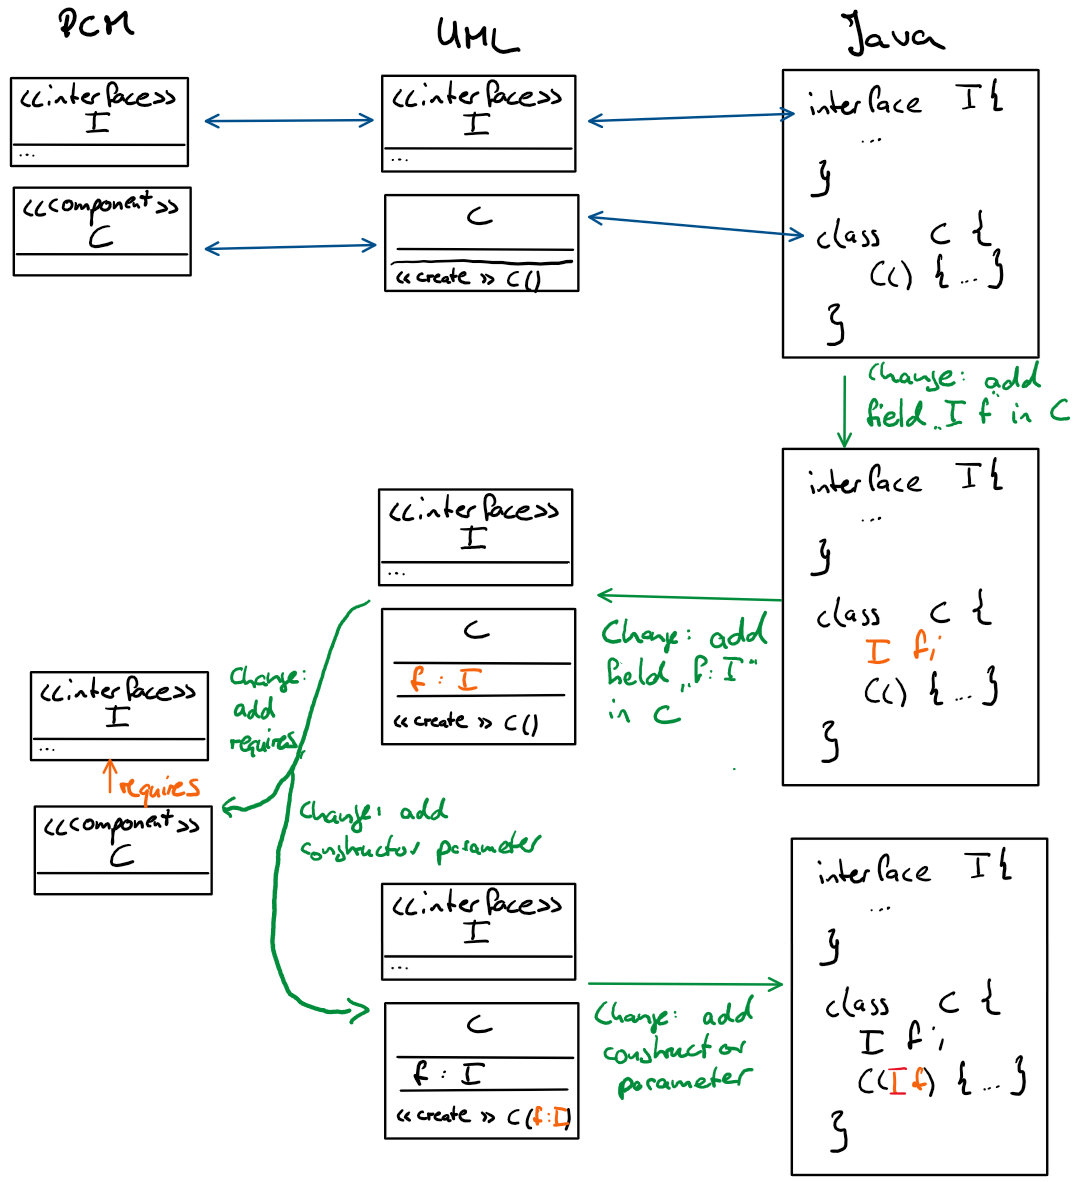
\includegraphics[width=\textwidth]{figures/correctness/orchestration/necessity_multiple_executions.png}
    \caption[Necessity of executing a transformation multiple times]{Necessity of executing a transformation multiple times. For initially consistent models, the Java code is changed, requiring the \acrshort{UML} and \acrshort{PCM} models to be updated accordingly. Blue lines without arrowheads connect initially corresponding elements, and green lines with arrowheads indicate changes performed by a user or consistency preservation.}
    \label{fig:orchestration:necessity_multiple_executions}
\end{figure}

\mnote{Example scenario for \gls{PCM}, \gls{UML} and Java}
Consider the example in \autoref{fig:orchestration:necessity_multiple_executions}, which depicts the introductory one of \autoref{fig:introduction:scenario_duplicate_execution} more precisely.
In the example, interfaces in the \gls{UML} and Java are related to architectural interfaces in a \gls{PCM} model.
\gls{PCM} components are realized by equally named classes in the \gls{UML} and Java.
Additionally, when a \gls{PCM} component requires an interface, this is realized by a field of the interface type and an appropriate constructor parameter in the component realization class in the \gls{UML} and Java.
Consistency is defined by transformations between \gls{PCM} and \gls{UML}, as well as between \gls{UML} and Java.

\mnote{Duplicate execution of transformation}
In the scenario in \autoref{fig:orchestration:necessity_multiple_executions}, we begin with a consistent state of one interface and component, each realized by an interface and class, respectively, in both the \gls{UML} and Java.
A user then introduces a change of the Java code, in which he or she adds a field of the interface type to the component realization class.
The transformation between \gls{UML} and Java propagates this change to the \gls{UML} model, such that both models are consistent again.
The transformation between \gls{PCM} and \gls{UML} then detects that the added field is of the type of an architectural interface, thus representing a requires relation between the corresponding component and the architectural interface. 
It adds the appropriate requires relation to the \gls{PCM} model but also adds an appropriate parameter to the constructor of the component realization class in the \gls{UML}.
This introduces a further inconsistency between the \gls{UML} and the Java model, which requires the transformation between \gls{UML} and Java to be executed again to also add that constructor parameter in the Java code.

\mnote{Cycles in transformation networks}
We have simplified the example to the necessary core, although in practice a further transformation between \gls{PCM} and Java may be required, e.g., to ensure that the field is set within the constructor.
One might argue that having such a cycle in the graph induced by the transformations between \gls{PCM}, \gls{UML}, and Java resolves the problem, as the second execution of the transformation between \gls{UML} and Java is not necessary if the information is propagated from the \gls{PCM} to Java.
This is, however, only true if exactly this execution order is chosen and if the transformation between \gls{PCM} and Java does not add further information to the Java model that must then be propagated to the \gls{UML}.

\mnote{Synchronizing transformations change already processed models}
In general, it is always possible that transformations need to react to the changes performed by other transformations if they are not in some way aligned with each other.
This is because a synchronizing transformation may change both models.
Thus, if one transformation restores consistency between two models and another transformation reacts to this by restoring consistency between one of these models and another one, then both these models become changed, which requires the first transformation to process the newly created changes again.

\begin{figure}
    \centering
    \newcommand{\distance}{13.8em}
\newcommand{\classwidth}{2em}

\begin{tikzpicture}

\umlclassvarwidth{A}{}{A}{
n
}{\classwidth}
\umlclassvarwidth[, right=\distance of A.north, anchor=north]{B}{}{B}{
n
}{\classwidth}
\umlclassvarwidth[, right=\distance of B.north, anchor=north]{C}{}{C}{
n
}{\classwidth}

\draw[consistency relation]
    ([yshift=0.7em]A.east)
    --
    node[pos=0, below right] {$a$}
    node[pos=1, below left] {$b$}
    node[above, align=center] {$\consistencyrelation{CR}{AB} = \{\tupled{a,b} \mid a.n, b.n \geq 0$ \\ 
        $\land \; b.n = a.n + 1 \land b.n \neq x\}$}
    ([yshift=0.7em]B.west);
\draw[consistency relation]
    ([xshift=0.7em]A.south)
    --
    node[pos=0, below left] {$a$}
    ++(0,-0.4*\distance)
    -|
    node[pos=1, below right] {$c$}
    node[above, pos=0.25] {$\consistencyrelation{CR}{AC} = \setted{\tupled{a,c} \mid a.n = c.n}$}
    ([xshift=-0.7em]C.south);
\draw[consistency relation]
    ([yshift=0.7em]B.east)
    --
    node[pos=0, below right] {$b$}
    node[pos=1, below left] {$c$}
    node[above, align=center] {$\consistencyrelation{CR}{BC} = \setted{\tupled{b,c} \mid b.n = c.n}$}
    ([yshift=0.7em]C.west);


\draw[transformation]
    ([yshift=-0.7em]A.east)
    --
    node[below, align=left] {$+a \xrightarrow{a.n \;\neq \; x-1} +b(n = a.n + 1)$\\
        $+b \xrightarrow{b.n \; \neq \; x} +a(n = b.n - 1)$}
    ([yshift=-0.7em]B.west);
\draw[transformation]
    ([xshift=-0.7em]A.south)
    --
    ++(0,-0.4*\distance-1.4em)
    -|
    node[below, pos=0.25, align=left] {$+a \rightarrow +c(n = a.n)$\\
        $+c \rightarrow +a(n = c.n)$}
    ([xshift=0.7em]C.south);
\draw[transformation]
    ([yshift=-0.7em]B.east)
    --
    node[below, align=left] {$+b \rightarrow +c (n = b.n)$\\
        $+c \rightarrow +b (n = c.n)$}
    ([yshift=-0.7em]C.west);

\end{tikzpicture}
    %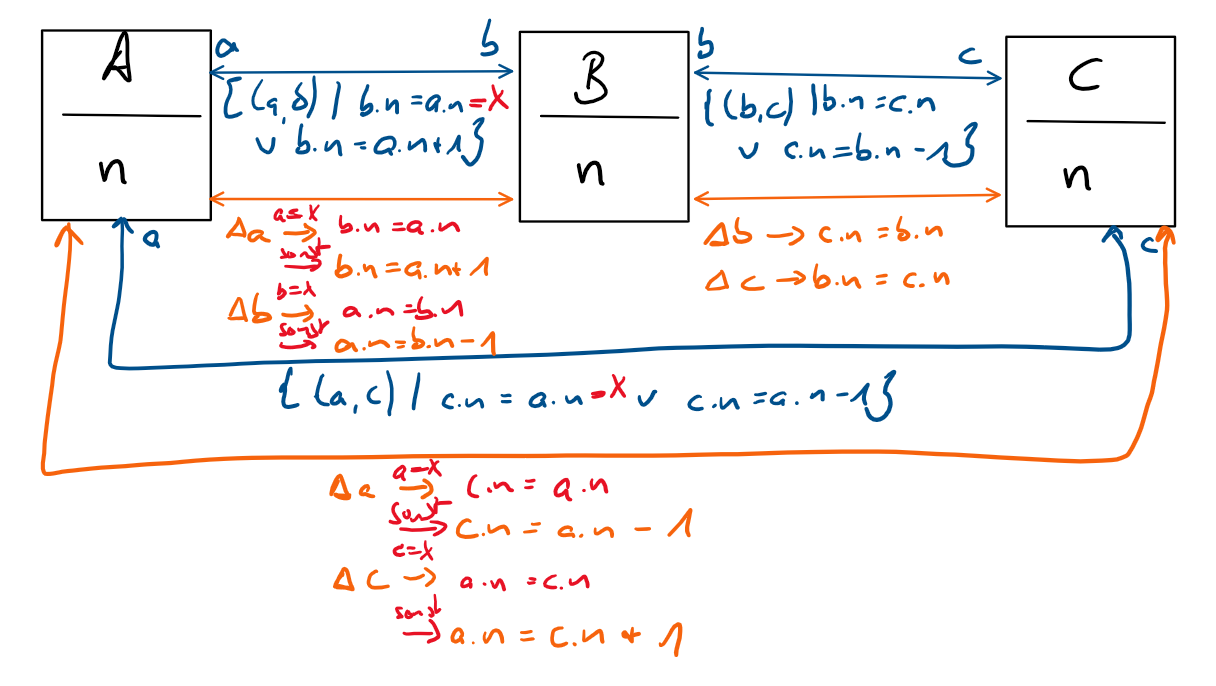
\includegraphics[width=\textwidth]{figures/correctness/orchestration/no_upper_bound_example.png}
    \caption[Example for arbitrary bounds of transformation execution]{Example of consistency relations and associated transformations with an arbitrary bound of necessary transformation executions depending on the value of $x$.}
    \label{fig:orchestration:no_upper_bound}
\end{figure}

\mnote{Example generalization}
We can generalize the previous example to the one of \autoref{fig:orchestration:no_upper_bound}.
It is an extension of the example given in \autoref{fig:synchronization:multiple_unidirectional_execution} for the necessity to execute the consistency preservation rules of a bidirectional transformation multiple times.
This also applies to the case in which multiple synchronizing transformations are combined.
The depicted relations and the sketched consistency preservation rules require that elements \modelelement{A}, \modelelement{B}, and \modelelement{C} with the same value of $n$ exist, and that for each \modelelement{A} with value $n$, a \modelelement{B} and \modelelement{C} with $n$ incremented by $1$ exist except for the case that $n = x-1$.
Thus, for an \modelelement{A} with $n = i$, all \modelelement{A}, \modelelement{B}, and \modelelement{C} with $i \leq n < x$ must exist.
This, obviously, requires the transformations to be executed $x-1-i$ times.

\mnote{Definition of example transformation network}
We prove the informally given statement with the following precise definition of the transformations for a fixed but arbitrary value of $x$.
Let \modelelement{A}, \modelelement{B}, and \modelelement{C} be the classes depicted in \autoref{fig:orchestration:necessity_multiple_executions}.
\parameterizeformat{
\begin{align*}
    & 
    \metamodelinstanceset{M}{1} \equalsperdefinition \mathcal{P}(\instances{\class{A}{}}), \;
    \metamodelinstanceset{M}{2} \equalsperdefinition \mathcal{P}(\instances{\class{B}{}}), \;
    \metamodelinstanceset{M}{3} \equalsperdefinition \mathcal{P}(\instances{\class{C}{}}) \\[0.5em]
    &
    \consistencyrelation{CR}{12} \equalsperdefinition \setted{\tupled{a,b} \in \instances{\class{A}{}} \times \instances{\class{B}{}} \mid a.n, b.n \ge 0 \land b.n = a.n + 1 \neq x}\\
    &
    \consistencyrelationset{CR}_{12} \equalsperdefinition \setted{\consistencyrelation{CR}{12}, \consistencyrelation{CR}{12}^T} \\
    &
    \consistencypreservationrule{\consistencyrelationset{CR}_{12}}^{\rightarrow}(\model{m}{1}, \model{m}{2}, \change{\metamodel{M}{1}}) \equalsperdefinition \change{\metamodel{M}{2}} \\
    & \formulaskip
    \withmath \change{\metamodel{M}{2}}(\model{m}{2}) \equalsperdefinition \setted{b \in \instances{\class{B}{}} \mid \exists a \in \change{\metamodel{M}{1}}(\model{m}{1}) : b.n = a.n + 1 \neq x} \\
    & 
    \consistencypreservationrule{\consistencyrelationset{CR}_{12}}^{\leftarrow}(\model{m}{2}, \model{m}{1}, \change{\metamodel{M}{2}}) \equalsperdefinition \change{\metamodel{M}{1}} \\
    & \formulaskip
    \withmath \change{\metamodel{M}{1}}(\model{m}{1}) \equalsperdefinition \setted{a \in \instances{\class{A}{}} \mid \exists b \in \change{\metamodel{M}{2}}(\model{m}{2}) : b.n = a.n + 1 \neq x \land a \geq 0} \\
    &
    \transformation{t}_{12} \equalsperdefinition \tupled{\consistencyrelationset{CR}_{12}, \consistencypreservationrule{\consistencyrelationset{CR}_{12}}^{\rightarrow}, \consistencypreservationrule{\consistencyrelationset{CR}_{12}}^{\leftarrow}} \\[0.5em]
    & 
    \consistencyrelation{CR}{13} \equalsperdefinition \setted{\tupled{a,c} \in \instances{\class{A}{}} \times \instances{\class{C}{}} \mid a.n = c.n}, \;
    \consistencyrelationset{CR}_{13} \equalsperdefinition \setted{\consistencyrelation{CR}{13}, \consistencyrelation{CR}{13}^T} \\
    & 
    \consistencypreservationrule{\consistencyrelationset{CR}_{13}}^{\rightarrow}(\model{m}{1}, \model{m}{3}, \change{\metamodel{M}{1}}) \equalsperdefinition \change{\metamodel{M}{3}} #2
    \withmath \change{\metamodel{M}{3}}(\model{m}{3}) \equalsperdefinition \setted{c \in \instances{\class{C}{}} \mid \exists a \in \change{\metamodel{M}{1}}(\model{m}{1}) : a.n = c.n} \\
    & 
    \consistencypreservationrule{\consistencyrelationset{CR}_{13}}^{\leftarrow}(\model{m}{3}, \model{m}{1}, \change{\metamodel{M}{3}}) \equalsperdefinition \change{\metamodel{M}{1}} #2
    \withmath \change{\metamodel{M}{1}}(\model{m}{1}) \equalsperdefinition \setted{a \in \instances{\class{A}{}} \mid \exists c \in \change{\metamodel{M}{3}}(\model{m}{3}) : a.n = c.n} \\
    & 
    \transformation{t}_{13} \equalsperdefinition \tupled{\consistencyrelationset{CR}_{13}, \consistencypreservationrule{\consistencyrelationset{CR}_{13}}^{\rightarrow}, \consistencypreservationrule{\consistencyrelationset{CR}_{13}}^{\leftarrow}} \\[0.5em]
    &
    \consistencyrelation{CR}{23} \equalsperdefinition \setted{\tupled{b,c} \in \instances{\class{B}{}} \times \instances{\class{C}{}} \mid b.n = c.n}, \;
    \consistencyrelationset{CR}_{23} \equalsperdefinition \setted{\consistencyrelation{CR}{23}, \consistencyrelation{CR}{23}^T} \\
    & 
    \consistencypreservationrule{\consistencyrelationset{CR}_{23}}^{\rightarrow}, \consistencypreservationrule{\consistencyrelationset{CR}_{23}}^{\leftarrow}, \andmath \transformation{t}_{23} \mathtextspacearound{accordingly} \\[0.5em]
    &
    \consistencyrelationset{CR} \equalsperdefinition \consistencyrelationset{CR}_{12} \cup \consistencyrelationset{CR}_{13} \cup \consistencyrelationset{CR}_{23} \\
    &
    \transformationset{T}_\mathvariable{inc} \equalsperdefinition \setted{\transformation{t}_{12}, \transformation{t}_{13}, \transformation{t}_{23}}
\end{align*}
}{}{\\ & \formulaskip}%

\mnote{Minimal number of executions in example}
For these transformations, we can show that the transformation $\transformation{t}_{12}$ needs to be executed a minimal number of times depending on $x$ for a specific input.
Thus, it is not sufficient to execute each transformation only once in this network, and, even worse, we can enforce the necessity for an arbitrary high number of executions by proper selection of $x$.

\begin{lemma}[Minimal Number of Transformation Executions]
    \label{lemma:minimal_executions}
    Let $\transformationset{T}_\mathvariable{inc}$ be the previously defined transformation set, let $\model{m}{1} = \model{m}{2}= \model{m}{3} = \emptyset$ be empty models, and let $\change{\metamodel{M}{1}} \in \changeuniverse{\metamodel{M}{1}}$ be a change with $\change{\metamodel{M}{1}}(\model{m}{1}) = \setted{a \in \instances{\class{A}{}} \mid a.n = 0}$.
    Then every orchestration function $\orcfunction{\transformationset{T}_\mathvariable{inc}}$ with $\appfunction{\orcfunction{\transformationset{T}_\mathvariable{inc}}}(\tupled{\model{m}{1},\model{m}{2},\model{m}{3}},\tupled{\change{\metamodel{M}{1}},\identitychange,\identitychange}) \consistenttomath \consistencyrelationset{CR}$ yields an orchestration that contains $\transformation{t}_{12}$ at least $x-1$ times.
\end{lemma}

\begin{proof}
    $\appfunction{\orcfunction{\transformationset{T}_\mathvariable{inc}}}$ can only return consistent models when it applies the transformations in the order delivered by $\orcfunction{\transformationset{T}_\mathvariable{inc}}$ by \autoref{def:applicationfunction}.
    We thus consider every orchestration, as delivered by any orchestration function, to show that it contains $\transformation{t}_{12}$ at least $x-1$ times to deliver consistent models.
    
    Let $\mathvariable{max}_n(\model{m}{1},\model{m}{2},\model{m}{3}) \equalsperdefinition \mathvariable{max}\setted{e.n \mid e \in \model{m}{1} \cup \model{m}{2} \cup \model{m}{3}}$ be the maximal value of $n$ among all instances of \modelelement{A}, \modelelement{B}, and \modelelement{C} in the given models $\model{m}{1}$, $\model{m}{2}$, and $\model{m}{3}$. In the following, we shortly note $\mathvariable{max}_n$ whenever the actual models are not relevant. We show three statements that together prove the lemma.

    \begin{properdescription}
        \item[Executing $\transformation{t}_{13}$ and $\transformation{t}_{23}$ does not increase $\mathvariable{max}_n$:]
        The transformations only ensure that for given models the returned models contain all elements with the same values of $n$ and do not introduce new elements with values of $n$ larger than the existing ones.
        \item[One execution of $\transformation{t}_{12}$ increases $\mathvariable{max}_n$ by at most $1$:]
        There is no \modelelement{A} or \modelelement{B} with $n > \mathvariable{max}_n$.
        For every \modelelement{A} with $n < \mathvariable{max}_n$, $\transformation{t}_{12}$ creates, if necessary, a \modelelement{B} with value $n + 1 \leq \mathvariable{max}_n$, thus not increasing $\mathvariable{max}_n$.
        For every \modelelement{B} with $n \leq \mathvariable{max}_n$, it creates, if necessary, an \modelelement{A} with value $n-1 < \mathvariable{max}_n$.
        For every \modelelement{A} with $n = \mathvariable{max}_n$, a \modelelement{B} with value $n+1 = \mathvariable{max}_n + 1$ is created, as long as $n \neq x-1$.
        For the newly created \modelelement{B}, no further elements need to be created to fulfill the relations.
        Thus, $\mathvariable{max}_n$ is, at most, increased by $1$.
        \item[$\mathvariable{max}_n(\model{m}{1},\model{m}{2},\model{m}{3}) < x-1 \Rightarrow \tupled{\model{m}{1},\model{m}{2},\model{m}{3}} \mathtextspacearound{inconsistent to} \consistencyrelationset{CR}$:]
        There is at least one element with $n = \mathvariable{max}_n$ within the models.
        If the element with $n = \mathvariable{max}_n$ is an \modelelement{A}, there must be a \modelelement{B} with value $n+1$ due to $\consistencyrelationset{CR}_{12}$ and $n < x-1$.
        But due to $n = \mathvariable{max}_n$ such a \modelelement{B} cannot exist, because otherwise $\mathvariable{max}_n = n+1$, so this is a contradiction. 
        If the element with $n = \mathvariable{max}_n$ is a \modelelement{C}, $\consistencyrelationset{CR}_{13}$ requires an \modelelement{A} with the same value of $n$ to exist and the same argument as before leads to a contradiction.
        Finally, if the element with $n = \mathvariable{max}_n$ is a \modelelement{B}, then because of $\consistencyrelationset{CR}_{23}$, a \modelelement{C} with the same value must exist and the same argument as before leads to a contradiction.
    \end{properdescription}

    In summary, we have shown that models $\model{m}{1}$, $\model{m}{2}$, and $\model{m}{3}$ are only consistent to $\consistencyrelationset{CR}$ when $\mathvariable{max}_n(\model{m}{1},\model{m}{2},\model{m}{3}) \geq x-1$.
    Additionally, only $\transformation{t}_{12}$ increases $\mathvariable{max}_n$ and with each execution it only increases it by at most $1$.
    In consequence, starting with $\mathvariable{max}_n = 0$, we need at least $x-1$ executions of $\transformation{t}_{12}$ in an arbitrary sequence of the transformations in $\transformationset{T}_\mathvariable{inc}$ to achieve consistent models.
\end{proof}

\mnote{Arbitrary number of necessary executions}
We have proven that transformation networks can require an arbitrary high number of executions of each transformation.
By selecting an appropriate $x$ in the example network, we can force the network to perform at least $x-1$ executions of one transformation to yield a consistent tuple of models.
With this insight, it directly follows that we cannot find an approach to define orchestration functions that deliver sequences containing each transformation only once if we want to ensure that the approach delivers a consistent orchestration of transformations if it exists. 

\begin{theorem}[Orchestration with Single Execution]
    \label{theorem:orchestration_single}
    For a set of transformations $\transformationset{T}$, there can be models $\modeltuple{m}$ and changes $\changetuple{}$ to them for which each possible orchestration function $\orcfunction{\transformationset{T}}$ with whom $\appfunction{\orcfunction{\transformationset{T}}}(\modeltuple{m}, \changetuple{})$ is consistent delivers a sequence as $\orcfunction{\transformationset{T}}(\modeltuple{m}, \changetuple{})$ that contains at least one transformation twice.
\end{theorem}

\begin{proof}
    According to \autoref{lemma:minimal_executions}, $\transformationset{T}_\mathvariable{inc}$ requires at least two executions of $\transformation{t}_{12}$ for the inputs in \autoref{lemma:minimal_executions} and $x \geq 3$.
    This proves the theorem by example.
\end{proof}

\mnote{Single execution insufficient}
Of course, for a specific set of transformations it may be possible that there is an orchestration for all possible models and changes to them leading to a consistent state and only requiring each transformation to be executed once.
\autoref{theorem:orchestration_single} shows, however, that this cannot be assumed in general.
If we execute each transformation only once, we may exclude cases for which multiple executions of transformations would have led to a consistent tuple of models.
The example we have given in \autoref{fig:orchestration:necessity_multiple_executions} is a simplification of a realistic transformation scenario, which we generalized to the previous network with transformations $\transformationset{T}_\mathvariable{inc}$.
For that reason, the insight is likely to be relevant in realistic scenarios.
We should not restrict orchestration to execute each transformation only once, as there can be realistic scenarios that require multiple executions to find consistent models.
In the following, we thus allow an arbitrary number of executions of each transformation.

\mnote{Authoritative models}
In addition, the examples, both the concrete one and the generalized abstract one, demonstrate that it can be necessary to modify the model that was originally changed by the user again.
This contradicts the notion of \emph{authoritative} models as, for example, introduced by \textcite{stevens2020BidirectionalTransformationLarge-SoSym}.
With that notion, specific models are defined authoritative and cannot be changed, for example, because they are immutable or because they were changed by the user, and reverting those changes shall be avoided.
While that behavior may be a desired, forbidding the modification of a whole model is not a proper solution as shown in the examples, which is why we do not consider a notion of authoritative models.


\subsection{Orchestration Function Behavior}
\label{chap:orchestration:problem:function_behavior}

\mnote{Returning $\bot$}
An application function is defined to return models only when they can be derived by applying transformations in an order delivered by the orchestration function and otherwise to return $\bot$.
In addition, we expect a \emph{correct} application function only to deliver consistent models.
We have, however, not yet defined under which conditions we expect the function not to return $\bot$, because there are different reasons why the function may not be able to deliver consistent models, although we could expect it to do so.
In fact, with the current definition, the function is even considered correct if it always returns $\bot$, which is obviously not practical.
Thus, we need to define when exactly we expect the function to return $\bot$.

\mnote{Reasons for not finding consistent orchestration}
It might be intuitive to expect an application function to always return consistent models when the input models are consistent and when there is an execution order of the transformations, i.e., an orchestration, that delivers consistent models.
This, in consequence, would lead to the requirement that the orchestration function delivers a sequence of transformations whose application delivers consistent models whenever such a sequence exists for the given models and changes to them.
There can be the following reasons why the orchestration function may not deliver such a sequence.
\begin{properdescription}
    \item[Incompatible Relations:] If the consistency relations are incompatible, a user change may introduce an element for which no consistent models exist. In consequence, the transformations cannot be executed in an order returning models that are consistent and still reflect the user change.
    \item[No Consistent Orchestration Exists:] Even if relations are compatible, transformations may be defined in a way that they make contradictory decisions for locally consistent solutions. Thus, for a given change the consistency relations provide different ways of restoring consistency, of which each transformation selects one that is not consistent to one of the other relations.
    Then, no order of the transformations can restore consistency, although consistent models exist for the given change.
    \item[No Consistent Orchestration Found:] Even if an order of transformations for given changes that delivers consistent models exists, the orchestration function may not deliver it. 
\end{properdescription}

\mnote{Implication hierarchy of reasons}
These reasons can be considered to reside at different levels, because each of them induces the next.
This means, if there is no orchestration, it cannot be found, and having contradictory relations, there exists no orchestration for some of the changes.
In the end, all of them lead to the situation that no orchestration can be found and, thus, the orchestration function is not able to deliver it.

\mnote{Assumption of consistent orchestration existence}
The intuitive requirement that the orchestration function delivers a consistent orchestration whenever it exists would ensure the third level and needs to assume fulfillment of the first two levels to avoid situations in which no consistent orchestration is found.
While we can assume compatibility of the relations, for which we proposed an analysis in \autoref{chap:compatibility}, we cannot assume that an orchestration does always exists, as we see in the following.

\mnote{Compatibility not ensuring consistent orchestration}
Although compatibility reduces the chance that an orchestration function does not deliver a consistent orchestration, as we have motivated with the scenario depicted in \autoref{fig:compatibility:unwanted_behavior}, it does not ensure that there is always such a sequence of transformations that the orchestration function can find.
In general, this is always the case when consistency relations define different options for consistency, i.e., if they allow the existence of different corresponding elements to consider the models consistent.
Compatibility ensures that there is an overlap of these corresponding elements, such that for every element, for which consistency is restricted, consistent models can be found.
If, however, the transformations always restore consistency by introducing corresponding elements that are not in this overlap, each transformation will restore consistency locally to its consistency relation, but they can, together, never restore consistency to all consistency relations.

\mnote{Overlapping options in consistency relations}
Consider the situation that we have three metamodels $\metamodel{A}{}$, $\metamodel{B}{}$, and $\metamodel{C}{}$ with instances $\model{a}{i}$, $\model{b}{k}$, and $\model{c}{l}$.
Let us assume that these models are uniquely indexed by $i$, $k$, and $l$, and that we defined the following \modellevelconsistencyrelations:
\begin{align*}
    &
    \consistencyrelation{CR}{AB} = \setted{\tupled{\model{a}{i}, \model{b}{k}} \mid k = i} \\
    &
    \consistencyrelation{CR}{AC} = \setted{\tupled{\model{a}{i}, \model{c}{l}} \mid l = i \lor l = i+1} \\
    &
    \consistencyrelation{CR}{BC} = \setted{\tupled{\model{b}{k}, \model{c}{l}} \mid l = k+1 \lor l = k+2}
\end{align*}
This induces the model tuples $\setted{\tupled{\model{a}{i}, \model{b}{k}, \model{c}{l}} \mid  i = k = l-1}$, which are consistent to all three consistency relations.
Thus, for any given model we are able to find instances of the other metamodels that are consistent to all consistency relations.
If we define consistency preservation rules for these consistency relations, the ones for $\consistencyrelation{CR}{AC}$ and $\consistencyrelation{CR}{BC}$ may decide between two models to restore consistency, because their conditions define two options for consistent models.
The set of consistent models, however, contains only those models fulfilling the first of these two conditions.
If each consistency preservation rule selects the models that fulfill the second condition, the resulting models are locally consistent to its consistency relation, but they will never become globally consistent to all three relations.
More precisely, if the consistency preservation rules for $\consistencyrelation{CR}{AC}$ select $\model{c}{i}$ for $\model{a}{i}$ and vice versa, and if the rules for $\consistencyrelation{CR}{BC}$ select $\model{c}{i+2}$ for $\model{a}{i}$ and vice versa, no orchestration of the transformations will yield consistent models, because they never select those models that are in the overlap of the consistency relations.

\begin{figure}
    \centering
    \newcommand{\distance}{24em}
\newcommand{\classwidth}{4em}

\begin{tikzpicture}

\umlclassvarwidth{person}{}{Person}{
firstname\\
lastname
}{\classwidth}
\umlclassvarwidth[, right=\distance of person.north, anchor=north]{resident}{}{Resident}{
name
}{\classwidth}
\umlclassvarwidth[, below right=0.4*\distance and 0.5*\distance of person.north, anchor=north]{employee}{}{Employee}{
name
}{\classwidth}

\draw[consistency relation] 
    ([yshift=-2.0em]person.north east)
    --
    node[pos=0, above right] {$p$}
    node[pos=1, above left] {$r$}
    node[below, align=center] {$\{\tupled{p,r} \mid \mathvariable{r.name} = \mathvariable{p.firstname} + "\text{\textvisiblespace}" + \mathvariable{p.lastname} $\\
    $\lor \mathvariable{r.name} = \mathvariable{p.lastname} + ",\text{\textvisiblespace}" + \mathvariable{p.firstname}\}$}
    ([yshift=-2.0em]resident.north west);
\draw[consistency relation] 
    ([xshift=0.7em]person.south)
    |-
    node[pos=0, below left] {$p$}
    node[pos=1, below left] {$e$}
    node[right, pos=0.35, align=center] {$\{\tupled{p,e} \mid\mathvariable{e.name} = \mathvariable{p.firstname} + "\text{\textvisiblespace}" + \mathvariable{p.lastname} $\\
    $\lor \mathvariable{e.name} = \mathvariable{p.lastname} + "\text{\textvisiblespace}"+ \mathvariable{p.firstname} \}$}
    ([yshift=0.7em]employee.west);
\draw[consistency relation] 
    ([xshift=-0.7em]resident.south)
    |-
    node[pos=0, below right] {$r$}
    node[pos=1, below right] {$e$}
    node[left, pos=0.22, align=center] {$\{\tupled{e,r} \mid \mathvariable{r.name} = \mathvariable{e.name}\}$}
    ([yshift=0.7em]employee.east);

\draw[transformation, -latex] 
    ([yshift=-0.8em]person.north east)
    --
    node[above=0.5em, align=center] {
        $+p \rightarrow r(\mathvariable{name} = \mathvariable{p.lastname} + ",\text{\textvisiblespace}" + \mathvariable{p.firstname})$\\[0.2em]
        $\begin{aligned}
            \mathtextspaceafter{\textup{Alternative 1:}} \;
            +r \rightarrow p(
            &
                \mathvariable{firstname} = \mathvariable{r.name.substringAfter}("\text{\textvisiblespace}")\\
            &
                \mathvariable{lastname} = \mathvariable{r.name.substringBeforeFirst}(",", "\text{\textvisiblespace}")
            )\\
            \mathtextspaceafter{\textup{Alternative 2:}}
            +r \rightarrow \mathvariable{if}(
            &
                \mathvariable{r.name.contains}(",")) \mathtextspacearound{then Alternative 1, else} \\
            p(
            &
                \mathvariable{firstname} = \mathvariable{r.name.substringBefore}("\text{\textvisiblespace}") \\
            &
                \mathvariable{lastname} = \mathvariable{r.name.substringAfter}("\text{\textvisiblespace}")
            )
        \end{aligned}$
    }
    ([yshift=-0.8em]resident.north west);
\draw[transformation, -latex] 
    ([xshift=-0.7em]person.south)
    |-
    node[below left=0.5em and 2.3em, pos=0.5, anchor=north west, align=center] {
        $\begin{aligned}
            +p \rightarrow +e(
            &
                \mathvariable{name} = \mathvariable{p.lastname} + "\text{\textvisiblespace}" + \mathvariable{p.firstname}
            ) \\
            +e \rightarrow +p(
            &
                \mathvariable{firstname} = \mathvariable{e.name.substringAfter}("\text{\textvisiblespace}")\\
            &
                \mathvariable{lastname} = \mathvariable{e.name.substringBefore}("\text{\textvisiblespace}")
            )
        \end{aligned}$
    }
    ([yshift=-0.7em]employee.west);
\draw[transformation, latex-]
    ([xshift=0.7em]resident.south)
    |-
    node[below right=0.5em and 2.3em, pos=0.5, anchor=north east, align=center] {
        $+e \rightarrow +r(\mathvariable{name} = \mathvariable{e.name})$\\
        $+r \rightarrow +e(\mathvariable{name} = \mathvariable{r.name})$
    }
    ([yshift=-0.7em]employee.east);


\node[consistency preservation element, below=5em of employee.south, anchor=north] (definitions) {
    $\begin{aligned}
    \mathtextspaceafter{\textup{with:}} \;
    & 
    \mathvariable{x.substringBefore}(\mathvariable{separator}) \equalsperdefinition \mathvariable{x.substring}(0, \mathvariable{x.indexOf}(\mathvariable{separator}))\\
    & 
    \mathvariable{x.substringBeforeFirst}(\mathvariable{separator1}, \mathvariable{separator2}) \equalsperdefinition\\
    &
    \formulaskip \mathvariable{x.substring}(\mathvariable{min}(\mathvariable{x.indexOf}(\mathvariable{separator1}), \mathvariable{x.indexOf}(\mathvariable{separator2})))\\
    & 
    \mathvariable{x.substringAfter}(\mathvariable{separator}) \equalsperdefinition \mathvariable{x.substring}(\mathvariable{x.indexOf}(\mathvariable{separator}) + 1)\\
    \end{aligned}$
};

\draw[lightgray] ([xshift=-1em, yshift=0.4em]definitions.north west) -- ([xshift=1em, yshift=0.4em]definitions.north east);


\end{tikzpicture}
    %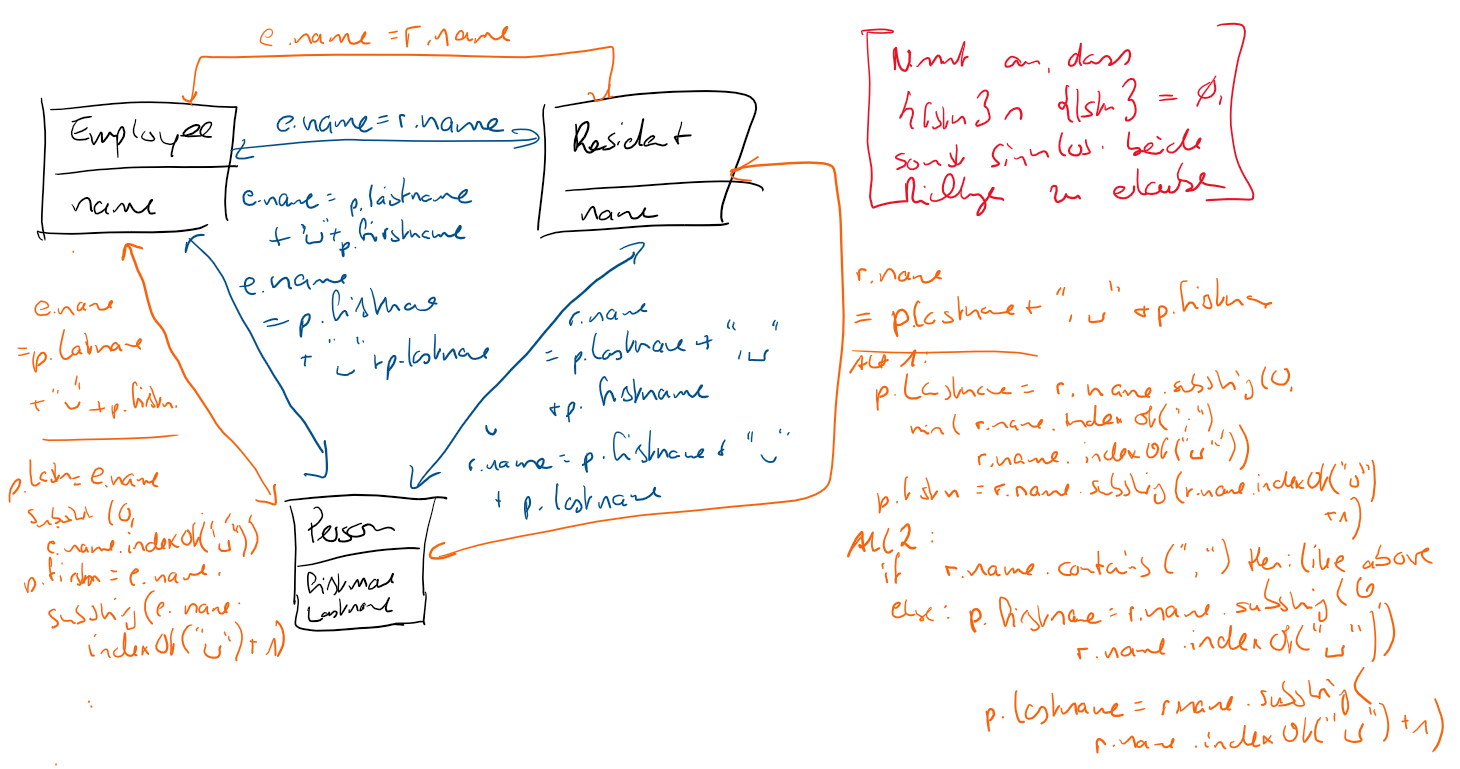
\includegraphics[width=0.85\textwidth]{figures/correctness/orchestration/no_orchestration.png}
    \caption[Consistency preservation rules without orchestration]{Consistency relations with options for corresponding elements leading to consistency preservation rules for which no consistent orchestration exists.}
    \label{fig:orchestration:no_orchestration}
\end{figure}

\mnote{Running example scenario}
\autoref{fig:orchestration:no_orchestration} demonstrates this situation at a derivation of the running example.
The consistency relation between employees and residents ensures that for each resident and employee there is a corresponding other element with the same $\mathvariable{name}$.
The consistency relations between employees and persons, as well as between residents and persons ensure that for each person there is a corresponding employee and resident, respectively, but they allow different relations of their names.
While both consider elements corresponding if the $\mathvariable{name}$ of an employee and resident, respectively, are the concatenation of the $\mathvariable{firstname}$ and $\mathvariable{lastname}$ of a person, an employee is also allowed to have the inverse concatenation of $\mathvariable{lastname}$ and $\mathvariable{firstname}$, whereas a resident is also allowed to have this inverse concatenation but with an additional separation of the $\mathvariable{lastname}$ and $\mathvariable{firstname}$ with a comma.
These options for the consistency relations provide further degrees of freedom for each transformation on its own, as they allow, for example, employee names to be encoded differently.
This can be reasonable if the order of $\mathvariable{firstname}$ and $\mathvariable{lastname}$ is not relevant in a model managing employees.
In combination with the other consistency relations, however, the only employees, residents, and persons that are considered consistent to all of the consistency relations are those having the same names with the concatenation of $\mathvariable{firstname}$ and $\mathvariable{lastname}$.
Nevertheless, these consistency relations are compatible, because for each possible condition element, i.e., for every possible employee, person, and resident, consistent models exist that contain them.

\mnote{Relations without consistent orchestration}
Consistency preservation rules for these consistency relations need to choose one of the given options for the names of corresponding employees, residents, and persons.
\autoref{fig:orchestration:no_orchestration} sketches consistency preservation rules that make such a selection.
The rules with alternative 1 ensure that for each employee, resident, and person corresponding elements exist, which fulfill those relations of the names that are conflicting.
This means, the employee's $\mathvariable{name}$ is the concatenation of the $\mathvariable{lastname}$ and $\mathvariable{firstname}$ of a person, whereas the resident's $\mathvariable{name}$ contains an additional comma in that concatenation.
In the other direction, the names of employees and residents are split at the appropriate indices given by the whitespace and comma, respectively, to calculate the required $\mathvariable{firstname}$ and $\mathvariable{lastname}$ of a person.
In consequence, there is no execution sequence of the transformations that results in consistent models, because the execution of the transformation between employees and persons always leads to a violation of the consistency relation between residents and persons and vice versa.
This is because the transformation between persons and residents always introduces a comma in the resident's $\mathvariable{name}$, which is then appended to the $\mathvariable{lastname}$ by the transformation between employees and persons.
A repeated execution of the transformation repeatedly appends that comma.
On the other hand, the execution of any of the transformations does never lead to the introduction of a person that fulfills the non-conflicting conditions of both consistency relations by simply containing a $\mathvariable{firstname}$ and $\mathvariable{lastname}$ that is represented as a concatenation of $\mathvariable{firstname}$ and $\mathvariable{lastname}$ in both an employee and a resident.
This is a concrete example for the abstract situation that of different options in consistency relations always the non-overlapping ones are chosen by the consistency preservation rules.

\mnote{Relations with consistent orchestration}
If we consider alternative 2 for the consistency preservation rule between persons and residents, we can always find a consistent orchestration.
The alternative rule decides how consistency is ensured based on the existence of a comma within the resident's $\mathvariable{name}$.
If a comma is present, the $\mathvariable{name}$ relation containing a comma is used, and otherwise the simple concatenation of $\mathvariable{firstname}$ and $\mathvariable{lastname}$ is assumed.
After adding an employee, first executing the transformation from employees to residents and afterwards the one from residents to persons ensures that all consistency relations are fulfilled, because the one between residents and persons sets the $\mathvariable{firstname}$ and $\mathvariable{lastname}$ of a person according to the relation that is also fulfilled between the person and the employee, because the $\mathvariable{name}$ does not contain a comma.
After adding a person, first executing the transformation from persons to employees and then the one from employees to residents results in an employee and a resident with inverse $\mathvariable{firstname}$ and $\mathvariable{lastname}$.
Since this resident is not consistent to the person, the transformation from residents to persons adds another person, which then also contains the swapped $\mathvariable{firstname}$ and $\mathvariable{lastname}$. Executing the same process again results in two persons, residents, and employees with both assignments of $\mathvariable{firstname}$ and $\mathvariable{lastname}$, which may not be intended but actually represents a consistent result.
Finally, after adding a resident we can, for example, first apply the transformation between residents and employees and then the one between residents and persons, resulting in consistent models due to the same reasons as above.

\mnote{Only specific orchestrations are consistent}
Although consistent orchestrations of the transformations with the consistency preservation rule defined as alternative 2 exist, not every execution order leads to consistent models.
In the scenarios discussed above, we have ensured that the transformation between residents and persons is executed after the addition of a resident.
If this transformation is executed after the addition of a person, a comma is added, which leads to the subsequent application of the same consistency preservation rules as with alternative 1 and implies that no further orchestration yields consistent models.

\mnote{Necessity to find consistent orchestrations}
No matter whether exactly these consistency relations and preservation rules for them may occur in an actual transformation network, they exemplify the general situation of having consistency preservation rules that select one of different options provided by the consistency relations to introduce corresponding elements to restore consistency.
The example shows that whether or not a consistent orchestration of transformations exists in such a situation depends on whether at least one transformation selects an option that is consistent to other consistency relations as well.
It also shows that even if a consistent orchestration exists, not all orchestrations yield consistent models.
Thus, we need to be able to find one that does.

\mnote{Resolvability}
In accordance with existing work~\cite{stevens2020BidirectionalTransformationLarge-SoSym}, we call a given tuple of models and changes \emph{resolvable} by a transformation network if a consistent orchestration exists.
%
%\mnote{Necessity to deal with unresolvability}
We have to accept that transformation networks may be unresolvable, i.e., that there is no consistent orchestration of the transformations.
Ensuring that a network is resolvable for every change would lead to restrictions for the individual transformations that would especially require different transformations to be aligned with each other.
Since that conflicts our assumption of independent development and modular reuse, we accept unresolvability and instead focus on how we can find an orchestration if it exists. 

\mnote{Optimality property of orchestration function}
In conclusion, we expect the application function to deliver consistent models whenever a consistent orchestration, i.e., an execution order that yields consistent models, exists.
Thus, we want to ensure that the orchestration function is able to always find such an orchestration if it exists.
We define this as an \emph{optimality} property in the following.


\subsection{Optimal Orchestration}

\mnote{Optimal orchestration function}
To ensure that an application function delivers consistent models whenever a consistent orchestration exists, we need to find an orchestration function that fulfills this property.
We denote this as an \emph{optimal} orchestration function.
Recall that $\generalizationfunction{\metamodeltuple{M},\transformation{t}}$ is the generalization function that applies a transformation to a model tuple that instantiates all metamodels in a tuple $\metamodeltuple{M}$.

\begin{definition}[Optimal Orchestration Function]
    Let $\transformationset{T}$ be a set of transformations for consistency relations $\consistencyrelationset{CR}$ and metamodels $\metamodeltuple{M}$.
    We say that an orchestration function $\orcfunction{\transformationset{T}}$ for these transformations is \emph{optimal} if, and only if, it returns a consistent orchestration whenever it exists:
    \begin{align*}
        &
        \forall \modeltuple{m} \in \metamodeltupleinstanceset{M} \mid \modeltuple{m} \consistenttomath \consistencyrelationset{CR} : 
        \forall \changetuple{\metamodeltuple{M}} \in \changeuniverse{\metamodeltuple{M}} : \\
        & \formulaskip
        \big[ 
            \exists \transformation{t}_{1}, \dots, \transformation{t}_{i} \in \transformationset{T} : 
            \exists \changetuple{\metamodeltuple{M}}' \in \changeuniverse{\metamodeltuple{M}} : 
            \big(
                \changetuple{\metamodeltuple{M}}'(\modeltuple{m}) \consistenttomath \consistencyrelationset{CR}\\
                & \formulaskip \formulaskip
                \land \generalizationfunction{\metamodeltuple{M}, \transformation{t}_{i}} \concatfunction \dots \concatfunction \generalizationfunction{\metamodeltuple{M}, \transformation{t}_{1}}(\modeltuple{m}, \changetuple{\metamodeltuple{M}}) = (\modeltuple{m}, \changetuple{\metamodeltuple{M}}')
            \big)
            \\
            & \formulaskip
            \Rightarrow
            \exists \transformation{t}_{1}', \dots, \transformation{t}_{k}' \in \transformationset{T} : 
            \exists \changetuple{\metamodeltuple{M}}'' \in \changeuniverse{\metamodeltuple{M}} : 
            \big(
                \changetuple{\metamodeltuple{M}}''(\modeltuple{m}) \consistenttomath \consistencyrelationset{CR}\\
                & \formulaskip \formulaskip
                \land \generalizationfunction{\metamodeltuple{M},\transformation{t}_{k}'} \concatfunction \dots \concatfunction \generalizationfunction{\metamodeltuple{M},\transformation{t}_{1}'}(\modeltuple{m}, \changetuple{\metamodeltuple{M}}) = (\modeltuple{m}, \changetuple{\metamodeltuple{M}}'') \\
                & \formulaskip \formulaskip
                \land \orcfunction{\transformationset{T}}(\modeltuple{m}, \changetuple{\metamodeltuple{M}}) = \sequenced{\transformation{t}_{1}', \dots, \transformation{t}_{k}'} 
            \big)
        \big]
    \end{align*}
\end{definition}

\mnote{Behavior without consistent orchestration existence}
Note that we allow an optimal orchestration function to return a sequence even when there is no consistent orchestration.
This is reasonable, because an application function may also support finding the reasons when no consistent orchestration is found by delivering a sequence of transformations that leads to a failure, as we discuss in \autoref{chap:orchestration:algorithm}.

\mnote{Application function optimality}
Finally, the result of the application function is what is relevant in the process of consistency preservation.
Thus, we apply the notion of \emph{optimality} to that function accordingly by requiring it to deliver consistent models whenever a consistent orchestration exists.

\begin{definition}[Optimal Application Function]
    \label{def:optimalapplicationfunction}
    Let $\transformationset{T}$ be a set of transformations for consistency relations $\consistencyrelationset{CR}$ and metamodels $\metamodeltuple{M}$.
    We say that an application function $\appfunction{\orcfunction{\transformationset{T}}}$ for these transformations is \emph{optimal} if, and only if, it returns models that are consistent whenever there is a consistent orchestration of the transformations:
    \begin{align*}
        &
        \forall \modeltuple{m} \in \metamodeltupleinstanceset{M} \mid \modeltuple{m} \consistenttomath \consistencyrelationset{CR} : 
        \forall \changetuple{\metamodeltuple{M}} \in \changeuniverse{\metamodeltuple{M}} : \\
        & \formulaskip
        \big[
            \exists \transformation{t}_{1}, \dots, \transformation{t}_{i} \in \transformationset{T} : 
            \exists \changetuple{\metamodeltuple{M}}' \in \changeuniverse{\metamodeltuple{M}} : 
            \big(
                \changetuple{\metamodeltuple{M}}'(\modeltuple{m}) \consistenttomath \consistencyrelationset{CR}\\
                & \formulaskip \formulaskip
                \land \generalizationfunction{\metamodeltuple{M}, \transformation{t}_{i}} \concatfunction \dots \concatfunction \generalizationfunction{\metamodeltuple{M}, \transformation{t}_{1}}(\modeltuple{m}, \changetuple{\metamodeltuple{M}}) = (\modeltuple{m}, \changetuple{\metamodeltuple{M}}')
            \big)
            \\
            & \formulaskip
            \Rightarrow \appfunction{\orcfunction{\transformationset{T}}}(\modeltuple{m},\changetuple{\metamodeltuple{M}}) \consistenttomath \consistencyrelationset{CR}
        \big]
    \end{align*}
\end{definition}

\mnote{Optimality dependency}
According to the defined behavior of an application function, an optimal application function requires an optimal orchestration function.

\begin{lemma}[Application / Orchestration Function Optimality]
    \label{lemma:optimalapplicationfunction}
    An application function $\appfunction{\orcfunction{\transformationset{T}}}$ can only be optimal if $\orcfunction{\transformationset{T}}$ is optimal.
\end{lemma}
\begin{proof}
    Let us assume that the condition in \autoref{def:optimalapplicationfunction} is fulfilled, i.e., that the input models are consistent and that a consistent orchestration of the transformations exists for them.
    Then, to be optimal, the application function needs to return models that are consistent.
    According to the definition of an application function (see \autoref{def:applicationfunction}), the sequence of transformations delivered by $\orcfunction{\transformationset{T}}$ for that input must yield the same model tuple as $\appfunction{\orcfunction{\transformationset{T}}}$.
    Thus, the orchestration function must deliver a sequence for such inputs that yields consistent models, which is equivalent to $\orcfunction{\transformationset{T}}$ being optimal.
\end{proof}


\subsection{The Orchestration Problem}

\mnote{Orchestration problem}
The problem to find a consistent orchestration whenever it is exists, i.e., to find an optimal orchestration function, is the central subject of the following sections.
This is what we denote as the \emph{orchestration problem}.
We prove that the problem is undecidable, discuss how we can make it decidable, and propose strategies to deal with its undecidability.
Finally, we come up with a discussion of conservatively approximating a solution to the problem.
We define the problem as follows.
\begin{definition}[Orchestration Problem]
    \label{def:orchestrationproblem}
    The problem to find a consistent orchestration of transformations for given inputs (models and changes to them) if it exists is called the \emph{orchestration problem}.
\end{definition}

\mnote{Orchestration existence problem}
Often, the more general problem of deciding whether a consistent orchestration exists is sufficient.
\begin{definition}[Orchestration Existence Problem]
    \label{def:orchestrationexistenceproblem}
    The question whether a consistent orchestration of transformations for given inputs (models and changes to them) exists is called the \emph{orchestration existence problem}.
\end{definition}

\mnote{Problem equivalence}
In fact, both these problems are equivalent in the sense that having a solution for one of them also delivers a solution for the other.
\begin{theorem}[Orchestration / Existence Problem Equivalence]
    \label{theorem:orchestrationproblemequivalence}
    The orchestration problem can be solved if, and only if, the orchestration existence problem can be solved.
\end{theorem}

\begin{proof}
    If a solution for the orchestration problem exists, it directly induces a solution for the orchestration existence problem, because if we find a consistent orchestration whenever it exists, we also know whether it exists.
    If a solution for the orchestration existence problem exists and we know that a consistent orchestration exists, we can find it by systematically testing all orchestrations of growing size until a consistent orchestration is found, since models are of finite size. Since we know that such an orchestration exists, this test must terminate, even though it may take an impractically long time.
\end{proof}

\mnote{Problem to optimality equivalence}
Since the orchestration problem is derived from the goal of finding an optimal application function, it is obviously equivalent to find an optimal application function or to solve the orchestration (existence) problem.

\begin{theorem}[Optimality / Orchestration Problem Equivalence]
    \label{theorem:optimal_application_function_orchestration_problem}
    An optimal application function $\appfunction{\orcfunction{\transformationset{T}}}$ can be defined if, and only if, a solution for the orchestration (existence) problem exists.
\end{theorem}

\begin{proof}
    We give the proof for the orchestration existence problem, which is, according to \autoref{theorem:orchestrationproblemequivalence}, equivalent to the orchestration problem.
    An optimal $\appfunction{\orcfunction{\transformationset{T}}}$ returns consistent models whenever there is a consistent orchestration.
    With such a function, we are able to decide whether such an orchestration exists or not.
    \begin{align*}
        \function{ExistsOrc}(\transformationset{T},\modeltuple{m},\changetuple{\metamodeltuple{M}}) \equalsperdefinition
            \begin{cases}
                \truemath, & \ifmath \appfunction{\orcfunction{\transformationset{T}}}(\modeltuple{m},\changetuple{\metamodeltuple{M}}) \consistenttomath \transformationset{T} \\
                \falsemath, & \otherwisemath
            \end{cases}
    \end{align*}
    $\function{ExistsOrc}$ returns \textsc{true} if, and only if, a consistent orchestration exists.
    Since $\appfunction{\orcfunction{\transformationset{T}}}$ is optimal, it returns consistent models in exactly those cases in which a consistent orchestration that yields them exists.

    If a solution for the orchestration existence problem exists, we know whether a consistent orchestration exists for an input.
    In that case, we can define $\appfunction{\orcfunction{\transformationset{T}}}$ to apply an according orchestration, which can be found by exhaustively testing different orchestration as discussed in the proof for \autoref{theorem:orchestrationproblemequivalence}, and otherwise to return $\bot$.
\end{proof}

